\chapter[Integración numérica]{Integración numérica%
\footnote{\licenseInfo}}
\label{cha:integracion-numerica}

El cálculo de una integral definida es un problema que aparece con
frecuencia, tanto en matemáticas como en otro ámbitos (ciencia,
ingeniería, economía,...). En concreto, dada una función
$f:[a,b]\subset\Rset\to\Rset$, se trata de aproximar numéricamente su
integral definida en $[a,b]$,
\begin{equation*}
  \int_a^bf(x)\,dx.
\end{equation*}

La necesidad de la aproximación numérica de integrales definidas
estriba en que, con frecuencia, resulta imposible (o demasiado costoso
computacionalmente) su cálculo de forma exacta. No sólo porque, en
contextos experimentales, la función podría venir dada por una tabla
de datos, sino porque la mayor parte de las funciones matemáticas no
son integrables mediante las técnicas usuales del cálculo elemental
y por tanto no resulta aplicable la regla de Barrow, $\int_a^b f(x)\,
dx=F(b)-F(a)$.

En este tema se plantearán métodos o fórmulas numéricas, llamadas
fórmulas de cuadratura, para la aproximación de $\int_a^b f(x)\,
dx$. La primera idea es la sustitución de $f(x)$ por un interpolador,
$p_n(x)$, de forma que $\int_a^bf(x)\,dx \approx \int_a^b p_n(x)\,
dx$. Esta última integral es fácil de calcular y, como veremos,
expresar como $\sum_{i=0}^n \omega_i \, f(x_i)$ (donde los coeficiente
$\omega_i$ provienen, por ejemplo, de la integración de las
funciones base de Lagrange).


Por tanto, las fórmulas de cuadratura para la aproximación de
$\int_a^b f(x)\, dx$ serán expresiones que utilizan los valores de la
función en un conjunto de $n+1$ \emph{nodos}, $\{x_0,x_1,\dots,x_n\}$,
multiplicados por $n+1$ \emph{pesos}
$\{\omega_0,\omega_1,\dots,\omega_n\}$:
\begin{definition}[Fórmula de cuadratura de tipo general]
  \label{def:formula-cuadratura}
  Una \resaltar{fórmula de cuadratura} (abreviadamente, f.c.) con
  $n+1$ nodos $\{x_i\}_{i=0}^n$ y pesos $\{\omega_i\}_{i=0}^n$ es una
  expresión del tipo:
  \begin{align}
    \label{eq:f.cuadratura}
    I_n(f)&=\sum_{i=0}^n \omega_i \, f(x_i).
    \\
    \intertext{Al valor}
    \notag
    E_n(f) &= \int_a^b f(x) - I_n(f) 
  \end{align}
  se le llama \resaltar{error} de la fórmula de cuadratura. 
  % donde $I_n(f)\in\Rset$ representa un valor aproximado de $\int_a^b
  % f(x)\,dx$ y $E_n(f)\in\Rset$ es el error que se comete en la
  % aproximación.
\end{definition}
Indicando que el error <<será pequeño>>, escribimos:
\begin{equation*}
  I_n(f) \approx \int_a^b f(x)\, dx.
\end{equation*}

\begin{definition}[Orden de una fórmula de cuadratura]
  \label{def:2}
  Una fórmula de cuadratura se dirá de \resaltar{orden} $m\in\Nset$ si
  verifica:
  \begin{align*}
    E_n(p)&=0 \quad \forall p\in\Pol_m[x] \text{ (polinomios
      de grado menor o igual que $m$) y}
    \\
    E_n(p)&\neq 0 \quad \text{para \emph{algún} polinomio }
    p\in\Pol_{m+1}[x] \text{ (de grado $m+1$)}.
  \end{align*}
\end{definition}
Así, decimos que una fórmula de cuadratura de orden $m$ es exacta para
los polinomios de orden (menor o igual a) $m$, pero no para los de
orden $m+1$.
\begin{remark}
  \label{rk:5}
  Utilizando la linealidad con respecto a $f$ de $\int_a^bf(x)\,dx$ y
  de $I_n(f)$, es evidente que una f.c. es de orden $m\in\Nset$ si
  y sólo si verifica:
  \begin{align*}
    E_n(x^k)&=0 \quad \forall k=0\dots,m \text{ y}
    \\
    E_n(x^{m+1})&\neq 0.
  \end{align*}
  Esta suele ser la forma de estudiar, en la práctica, el orden de una
  fórmula de cuadratura.
\end{remark}

\begin{example}
  \label{ex:formula-punto-medio}
  La siguiente fórmula de cuadratura de un punto ($n=0$) es conocida
  como \resaltar{fórmula del punto medio},
  \begin{equation}
    \label{eq:f.c.-pto-medio}
    I_0(f)= (b-a) f\left(\frac{a+b}{2}\right),
  \end{equation}
  y tiene orden $1$. En efecto, evaluando $E_0(x^k)=\int_a^b
  x^k\, dx-I_0(x^k)$ para $k\ge 0$:
  \begin{align*}
   \text{Para } k&=0:\ E_0(1) = \int_a^b 1\cdot dx - (b-a)\cdot 1 = 0.
   \\
   \text{Para } k&=1:\ E_0(x) = \int_a^b x\cdot dx - (b-a)\frac{a+b}{2}
   = \frac{1}{2}(b^2-a^2) -  (b-a) \frac{a+b}{2} = 0.
   \\
   \text{Para } k&=2:\ E_0(x^2) = \int_a^b x^2\cdot dx 
   - (b-a) \frac{(a+b)^2}{4} 
   = \frac{1}{3}(b^3-a^3) - (b-a)\frac{(a+b)^2}{4} 
   \neq 0.
  \end{align*}
\end{example}

\begin{example}
  \label{ex:formula-trapecio}
  La siguiente f.c. de dos puntos ($n=1$) es conocida
  como \resaltar{fórmula del trapecio}:
  \begin{equation*}
    I_1(f)= \frac{b-a}{2}\left(f(a)+f(b)\right).
  \end{equation*}
  La formula del trapecio es de orden 1:
  \begin{align*}
    \text{Para } k&=0:\ E_1(1) = (b-a) - \frac{b-a}2\cdot 2 = 0.
    \\
    \text{Para } k&=1:\ E_1(x) = \frac{b^2-a^2}{2} -
    \frac{(b-a)}{2}(a+b) = 0.
    \\
    \text{Para } k&=2:\ E_1(x^2) = \frac{b^3-a^3}{3} -
    \frac{(b-a)}{2}(a^2+b^2) \neq 0.
  \end{align*}
\end{example}

\begin{example}
  \label{ex:formula-simpson}
  La \resaltar{fórmula de Simpson} es la siguiente f.c.
  de tres puntos ($n=2$):
  \begin{equation}
    I_2(f)= \frac{b-a}{6}\left[f(a)+f
      \left(\frac{a+b}{2}\right)+f(b)\right].
    \label{eq:formula-simpson}
  \end{equation}
  Su orden es $3$. La demostración es similar a los ejemplos anteriores.
\end{example}

\section{Fórmulas de cuadratura de tipo interpolatorio}
\label{sec:cuadratura-interpolatorio}

La expresión~(\ref{eq:f.cuadratura}) define a una fórmula de
cuadratura de tipo general, para pesos $\omega_i$ y nodos $x_i$
cualesquiera, no necesariamente provenientes de la interpolación.
Pero por motivos que veremos luego
(proposición~\ref{pro:existencia.fcti}), nos interesarán especialmente
aquellas fórmulas de cuadratura que vengan dadas por integración de un
polinomio de interpolación.
\begin{definition}[Fórmula de cuadratura de tipo interpolatorio]
  Sea $f\in C^0([a,b])$ y sea $p_n$ el polinomio de interpolación de
  Lagrange asociado a $f$ y a $n+1$ nodos
  $\{x_0,x_1,\dots,x_n\}$. Diremos que una f.c. es de tipo
  interpolatorio si 
  \begin{equation}
    \label{eq:fcti}
    I_n(f)=\int_a^b p_n(x)\, dx.
  \end{equation}
  \label{def:fcti}
\end{definition}

La expresión~(\ref{eq:fcti}) se puede escribir de la forma
de~(\ref{eq:f.cuadratura}), es decir como suma de $f(x_i)$ por
cierto pesos. En efecto, dada $f\in C^0([a,b])$, podemos escribir
$p_n$ usando la fórmula de interpolación de Lagrange:
\begin{equation*}
  p_n(x)=\sum_{i=0}^n f(x_i) L_i(x),
\end{equation*}
donde $\{L_i\}_{i=0}^n$ es la base de Lagrange asociada a
$\{x_i\}_{i=0}^n$. Por lo tanto,
\begin{equation*}
  \int_a^bp_n(x)\,dx = \sum_{i=0}^n f(x_i) \int_a^b L_i(x)\,dx 
  =\sum_{i=0}^n \omega_i f(x_i), \quad \text{con } \omega_i=\int_a^b L_i(x)\,dx.
\end{equation*}

\begin{example}
  \label{ex:formula-pto-medio-interpol}
  La f.c. del punto medio~(\ref{eq:f.c.-pto-medio}) es de tipo
  interpolatorio. En efecto, si $p_0(x)$ es el polinomio de 
  interpolación de grado cero asociado a $f$ en $x_0=(a+b)/2$, es
  decir $p_0(x)=f(x_0)$ para todo $x\in[a,b]$, entonces:
  \begin{equation*}
    I_0(f) = (b-a)f\left(\frac{a+b}{2}\right) = \int_a^b p_0(x)\,dx.
  \end{equation*}
\end{example}

\begin{example}
  \label{ex:formula-trapecio-interpol}
  Fijamos $n=1$, $x_0=a$ y $x_1=b$. Buscamos coeficientes, $\omega_0$
  y $\omega_1$ tales que la siguiente fórmula de cuadratura sea de
  tipo interpolatorio:
  \begin{equation*}
    I_1(f)=\omega_0 f(x_0) + \omega_1 f(x_1).
  \end{equation*}
  Según la definición~\ref{def:fcti}, esto significa que
  \begin{equation*}
    I_1(f)=\int_a^b p_n(x)= 
    \underbrace{\left(\int_a^bL_0(x)\right)}_{\omega_0} f(x_0)+
    \underbrace{\left(\int_a^bL_1(x)\right)}_{\omega_1} f(x_1).
  \end{equation*}
  Como
  \begin{equation*}
    L_0(x)=\frac{x-x_1}{x_0-x_1}=\frac{x-b}{a-b} \quad \text{y} \quad
    L_1(x)=\frac{x-x_0}{x_1-x_0}=\frac{x-a}{b-a},
  \end{equation*}
  entonces
  \begin{equation*}
    \omega_0 = \int_a^b \frac{x-b}{a-b} = \frac{-(a-b)^2}{2(a-b)}=\frac{b-a}{2},
    \quad
    \omega_1 = \int_a^b \frac{x-a}{b-a} = \frac{(b-a)^2}{2(b-a)}=\frac{b-a}{2}.
  \end{equation*}
  Es decir, que la fórmula de cuadratura que buscamos es la
  fórmula del trapecio:
  \begin{equation*}
    I_1(f)=\frac{b-a}{2}
    \left(
      f(a)+f(b)
    \right).
  \end{equation*}
\end{example}

\begin{example}
  La fórmula de Simpson~(\ref{eq:formula-simpson}) es de tipo
  interpolatorio. La demostración se deja como ejercicio.
\end{example}

La siguiente proposición afirma que las f.c.t.i. son óptimas, en el
sentido de que son las f.c. de mayor orden.
\begin{proposition}
  \label{pro:existencia.fcti}
  Dados $n+1$ nodos distintos, $x_0<x_1<\cdots<x_n$:
  \begin{enumerate}
  \item Sobre estos nodos existe una única f.c. con orden $\ge
    n$.
  \item Esta f.c. coincide con la f.c.t.i. correspondiente a
    $\{x_i\}_{i=0}^n$.
  \end{enumerate}
\end{proposition}
\begin{proof}~\par
  \punto{1} Sea $I_n(f)=\sum_{i=0}^n \omega_i f(x_i)$ una
  f.c. cualquiera sobre $\{x_i\}_{i=0}^n$. $I_n(f)$ tiene orden $\ge
  n$ si y solo si $E(x^k)=0$ para $k=0,\dots,n$. Escribiendo estas $n+1$
  ecuaciones,
  \begin{equation}
    \left.
  \begin{alignedat}{2} % 2 bloques de columnas rl
    E(1)&=0 \quad \Leftrightarrow\ \quad &
    \omega_0 + \omega_1 + \cdots \omega_n &=
    \int_a^b 1\cdot\,dx = b-a
    \\
    E(x)&=0 \quad \Leftrightarrow\ \quad &
    \omega_0 x_0 + \omega_1 x_1 + \cdots \omega_n x_n &=
    \int_a^b x \cdot\,dx = \frac{b^2-a^2}{2}
    \\
    &\ \, \vdots & &\ \, \vdots
    \\
    E(x^n)&=0 \quad \Leftrightarrow\ \quad &
    \omega_0 x_0^n + \omega_1 x_1^n + \cdots \omega_n x_n^n &=
    \int_a^b x^n \cdot\,dx = \frac{b^{n+1}-a^{n+1}}{n+1}
    \\
  \end{alignedat}
  \right\}
  \label{eq:sl.fcti}
\end{equation}
  tenemos un sistema lineal con $n+1$ incógnitas
  $\{\omega_i\}_{i=0}^n$. La matriz asociada, es la conocida matriz de
  Vandermonde, 
  \begin{equation*}
    A =
    \begin{pmatrix}
      1 & x_0& \cdots & x_0^n \\
      1 & x_1& \cdots & x_1^n \\
      \vdots & \vdots & & \vdots \\
      1 & x_n& \cdots & x_n^n 
    \end{pmatrix}
  \end{equation*}
  que fue estudiada en el teorema~\ref{thm:existencia-unicidad-lagrange}
  (existencia y unicidad del polinomio de interpolación de Lagrange),
  donde comprobamos que $A$ no es singular si los nodos son distintos.
  Por lo tanto, existe una única solución, $\{\omega_i\}_{i=0}^n$, que
  determina la única f.c. $I_n(f)$ de orden $\ge n$.

  \punto{2} Veamos que esta única f.c. de orden $\ge n$ coincide con
  la f.c.t.i. correspondiente a $\{x_i\}_{i=0}^n$. Para ello, basta
  comprobar que la f.c.t.i. definida sobre nodos $\{x_i\}_{i=0}^n$
  tiene orden al menos $n$. 
  Pero esto es evidente: sea $I_n(f)=\int_a^b p_n(x)\, dx$ donde $p_n$
  interpola a $f$ en los nodos $\{x_i\}_{i=0}^n$. Si $f(x)=p(x)$ es un
  polinomio de grado $\le n$, entonces su polinomio de interpolación
  de Lagrange es $p_n(x)=p(x)$ (por unicidad), por tanto
  $E_n(p)=\int_a^b p(x)\,dx - \int_a^b p_n(x)\,dx =0$.
\end{proof}

\begin{remark}
  \label{rk:6}
  La demostración de la proposición anterior nos proporciona una forma
  de calcular los pesos de cualquier f.c.t.i.: resolver el sistema
lineal~(\ref{eq:sl.fcti}). Este método se conoce como \resaltar{método de
  los coeficientes indeterminados}. Tiene el inconveniente de que su
matriz asociada, la matriz de Vandermonde, está mal condicionada
  cuando $n\to\infty$.
\end{remark}

\begin{example}
  \label{ex:coef-indetermin:formula-trapecios-abierta}
  Utilizaremos el método de los coeficientes indeterminados para
  calcular los pesos de la fórmula de cuadratura en $[a,b]$ que es de
  mayor orden (es decir, la f.c.t.i.) para los nodos $x_0=a+h$ y
  $x_1=a+2h$, con $h=\frac{b-a}{3}$.
  
  Para $n=1$, obtenemos el siguiente sistema:
  \begin{align*}
    \omega_0 + \omega_1 &= b-a,
    \\ 
    x_0\omega_0 + x_1\omega_1 &= \frac{b^2-a^2}{2},
  \end{align*}
  cuya única solución es:
  \begin{equation*}
    \omega_0=\omega_1=\frac{3h}{2}
  \end{equation*}
  Así obtenemos la siguiente fórmula de cuadratura (que es conocida
  como \textit{fórmula de los trapecios abierta}:
  \begin{equation*}
    I_1(f)=\frac{3h}{2}
    \left(
      f(x_0)+f(x_1),
    \right)
    \quad \text{con } x_0=a+h, \ x_1=a+2h,
  \end{equation*}
  para $h=\frac{b-a}{3}$.
\end{example}

\subsection*{Cota del error en fórmulas de tipo interpolatorio}

Sea $I_n(f)$ una f.c.t.i. sobre $n+1$ puntos y sea $p_n$ el polinomio
de Lagrange asociado.  Utilizando la
expresión~(\ref{eq:expresion-error-interpol}) de error de
interpolación del polinomio de Lagrange podemos razonar como sigue:

\begin{align*}
  E_n(f)=&\int_a^b f(x)\, dx - I_n(f) =
  \int_a^b\left(f(x)-p_n(x)\right)\,dx 
  \\
  =&\int_a^b \frac{f^{n+1)}(\xi_x)}{(n+1)!} (x-x_0)(x-x_1)\dots(x-x_n) \,dx
  \le \int_a^b  \frac{M_{n+1}}{(n+1)!} (b-a)^{n+1} \, dx,
\end{align*}
donde $M_{n+1}=\max_{x\in [a,b]} |f^{n+1)}(x)|$.
Por lo tanto toda f.c.t.i con $n+1$ puntos en un intervalo $[a,b]$
verifica la siguiente cota del error:
\begin{equation}
  E_n(f) \le  \frac{M_{n+1}}{(n+1)!} (b-a)^{n+2}.
  \label{eq:cota-error-fcti}
\end{equation}

Tal y como en el capítulo~\ref{cha:Interpolacion-aproximacion}, nos
podemos preguntar: dada una f.c.t.i., para una función $f$
suficientemente regular (por ejemplo infinitamente derivable),
¿podemos garantizar que $E_n(f)$ tiende a cero cuando $n\to\infty$?,
es decir,
\begin{eqnarray*}
  \text{\large ¿ \;} 
  \lim_{n\to\infty} \int_a^b p_n(x) = \int_a^bf(x)
  \text{\; \large?}
  \label{eq:pregunta.p_n.to.f}
\end{eqnarray*}
Una vez más, la respuesta a esta pregunta es negativa, en general, como
sugiere el hecho de que en la estimación~(\ref{eq:cota-error-fcti}) no
resulta posible acotar el término $M_{n+1}$, para cualquier función
infinitamente derivable, cuando $n\to\infty$.

Sin embargo, si denotamos $h=(b-a)$, la
cota~(\ref{eq:cota-error-interpol-1}) nos garantiza que $E_n(f)$
converge a cero cuando $h\to 0$. De hecho, si utilizamos la notación
%$g(h)=O(h^m)$ para expresar que
\begin{align*}
  g(h)=O(h^m) \quad&\Longleftrightarrow\quad\lim_{h\to 0} \frac{g(h)}{h^m}=C
\qquad \text{($C\in \Rset$ constante)},
%
\intertext{entonces}
%
E_n(f)&=O(h^{n+2}).
\end{align*}

Por este motivo, en la práctica se suelen utilizar f.c. compuestas, en
las que dividimos $[a,b]$ en subintervalos de integración de modo que
$h\to 0$ (ver sección~\ref{sec:fc-compuestas}).

\section{Fórmulas de Newton-Côtes}
\label{sec:formulas-de-newton}

\begin{definition}
  \label{def:1}
  Se denomina fórmula de cuadratura de Newton-Côtes (abreviadamente
  N-C) a toda aquella f.c.t.i cuyas abscisas se encuentran
  uniformemente espaciadas (es decir, $x_{i}-x_{i-1}=h$ para todo
  $i=1,\dots,n$. Existen dos tipos:
  \begin{itemize}
  \item Fórmulas cerradas: aquellas en las que
    \begin{align*}
      x_0=a, \quad x_n=b, \quad x_i=x_0 + ih,
     \quad 
     \text{con } h=\frac{b-a}{n}.
    \end{align*}
  \item Fórmulas abiertas: aquellas en las que
    \begin{align*}
      x_0=a+h, \quad x_n=b-h, \quad x_i=x_0 + ih,
     \quad 
     \text{con } h=\frac{b-a}{n+2}.
    \end{align*}
  \end{itemize}
\end{definition}

\begin{theorem}
  \label{thm:error.formulas-nc}
  Sea $I_n$ una f.c.t.i. sobre $n+1$ puntos equiespaciados en
  $[a,b]$. Supongamos que $f\in C^k([a,b])$, donde $k=n+2$ si $n$ es par
  y $k=n+1$ si $n$ es impar. Entonces, existe $\xi\in(a,b)$ tal que
  \begin{equation}
  \label{eq:error-formulas-nc} 
  E_n(f)=\int_a^bf(x)\,dx - I_n(f)
    = \gamma_n h^{k+1} \frac{}{k!}f^{k)}(\xi),
  \end{equation}
  siendo:
  \begin{itemize}
  \item Si $I_n$ es una fórmula cerrada: $h=(b-a)/n$ y
    \begin{align*}
      \text{ si $n$ es par }
      \gamma_n=\int_0^n t \Pi_n(t) dt,
      \quad \text{si $n$ es impar }
          \gamma_n=\int_0^n \Pi_n(t) dt.
    \end{align*}
  \item Si $I_n$ es una fórmula abierta: $h=(b-a)/(n+2)$ y
    \begin{align*}
      \text{si $n$ es par }
      \gamma_n=\int_{-1}^{n+1} t \Pi_n(t) dt,
      \quad \text{si $n$ es impar }
      \gamma_n=\int_{-1}^{n+1} \Pi_n(t) dt.
    \end{align*}
  \end{itemize}
  En lo anterior se ha usado la notación:
  $\Pi_n(t)=(t)=t(t-1)(t-2)\cdots (t-n)$.
\end{theorem}

\begin{remark}~
  \label{rk:7}
  \begin{enumerate}
  \item Según la expresión del error en el teorema anterior, el error
    es cero para polinomios de grado menor o igual a $k$ (pues se
    anula la derivada), por tanto las fórmulas de Newton-Côtes son
    exactas para polinomios de grado $k$ ($k=n+1$ ó $n+2$), en
    concreto:
    \begin{enumerate}
    \item Si $n$ es \textit{par}, las fórmulas de N--C son de 
      orden $n+2$.
    \item Si $n$ es \textit{impar}, las fórmulas de N--C son de 
      orden $n+1$.
    \end{enumerate}
  \item Aunque una primera impresión puede sugerir que las fórmulas de
    N-C abiertas y cerradas tienen el mismo orden, no hay que olvidar
    que el valor de $h$ difiere entre ellas.
 Si queremos comparar el
    error entre fórmulas abiertas y cerradas, debemos utilizar el
    mismo valor de $h$.
    
    Fijemos un paso $h=(b-a)/p$, con cierto $p\in\Nset$. Entonces éste
    se corresponde con una fórmula cerrada de $n=p+1$ puntos o con una
    fórmula abierta de $n=p-1$ puntos. Así, en la expresión del error:
    \begin{enumerate}
    \item En las fórmulas \emph{abiertas}:\par
      \begin{tabular}{rl}
      Si $p$ es par, entonces $n$ es impar y: &$k=n+1=p$
      \\
      Si $p$ es impar, entonces $n$ es par y: &$k=n+2=p+1$
    \end{tabular}
    \item En las fórmulas \emph{cerradas}:\par
      \begin{tabular}{rl}
      Si $p$ es par, entonces $n$ es impar y: &$k=n+1=p+2$
      \\
      Si $p$ es impar, entonces $n$ es par y: &$k=n+2=p+3$
    \end{tabular}
    \end{enumerate}
    Como conclusión: fijado un mismo paso $h$, en todos los casos
    \emph{el orden de las fórmulas cerradas es superior en dos
      unidades al de las fórmulas abiertas}.
  \end{enumerate}
\end{remark}
\begin{example}[Fórmulas de cuadratura abiertas]
  Consideremos $n+1$ puntos en un intervalo cualquiera,
  $[a,b]=[x_{0},x_{n}]$ y $f_k=f(x_k)$, $k=0,\dots,n$. Un simple
  cálculo nos permite calcular los pesos de la f.c. (bien sea mediante
  integración de las funciones base de Lagrange, como en los
  ejemplos~\ref{ex:formula-pto-medio-interpol}
  y~\ref{ex:formula-trapecio-interpol} o bien usando el método de los
  coeficiente indeterminados, como en el
  ejemplo~\ref{ex:coef-indetermin:formula-trapecios-abierta}) y las
  constantes $\gamma_n$ anteriores para $n=1,2,3,...$.

  Por ejemplo, para $n=1$, tendremos $[a,b]=[x_0,x_1]$. La f.c.t.i
  asociada es la fórmula de los trapecios (ver
  ejemplo~\ref{ex:formula-trapecio-interpol}):
  \begin{equation*}
    I_1(f) = \int_{a}^{b} \frac{b-a}{2}(f(a)+f(b)) 
    = \int_{x_0}^{x_1} \frac{h}{2}(f_0+f_1)
  \end{equation*}
  y el error viene dado por~(\ref{eq:error-formulas-nc}). En este
  caso, como $n$ es impar, $k=n+1=2$ y así
  \begin{equation*}
    E_n(f)=\gamma_1 h^{3}\frac{f^{2)}(\xi)}{2}=\frac{-h^3}{12} f^{2)}(\xi),
  \end{equation*}
  donde se ha usado que, según el Teorema~\ref{thm:error.formulas-nc},
  para una f.c. cerrada con $n=1$:
  \begin{equation*}
    \gamma_1 = \int_0^1 \Pi_1(t)\,dt = \int_0^1 t(t-1) = \frac{-1}{6}.
  \end{equation*}
  
  Despejando $\int_a^b f(x)\,dx$ en~(\ref{eq:error-formulas-nc}) se
  puede condensar lo anterior en:
  \begin{equation*}
    \int_a^b f(x)\,dx = \int_{x_0}^{x_1} f(x)\,dx =
    \int_{x_0}^{x_1} \frac{h}{2}(f_0+f_1) - \frac{h^3}{12} f^{2)}(\xi).
  \end{equation*}

  Procediendo análogamente para $n=2,3,4,5$, se tiene las
  siguiente tabla de fórmulas de cuadratura de N--C cerradas:
  \begin{center}
    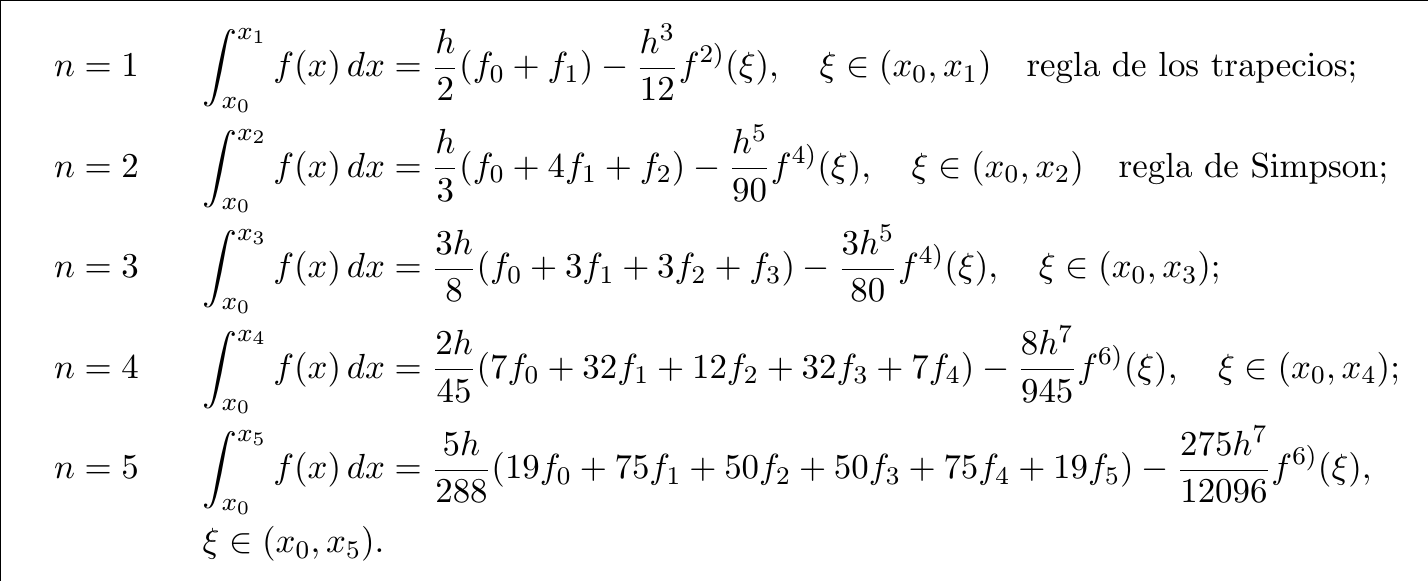
\includegraphics[width=0.95\linewidth]{tema3/formulas-nc-cerradas}
  \end{center}
\end{example}

\begin{example}[Fórmulas de cuadratura abiertas]
  Sean $x_0,x_1,\cdots,x_n$ los $n+1$ puntos interiores al intervalo
  $[a,b]$ en una f.c. de N--C abierta. Denotemos ahora $x_{-1}=a$,
  $x_{n+1}=b$ y $f_k=f(x_k)$, $k=0,\dots,n$. Procediendo como antes
  se tienen las siguientes fórmulas junto con las expresiones de error
  asociadas:
  \begin{center}
    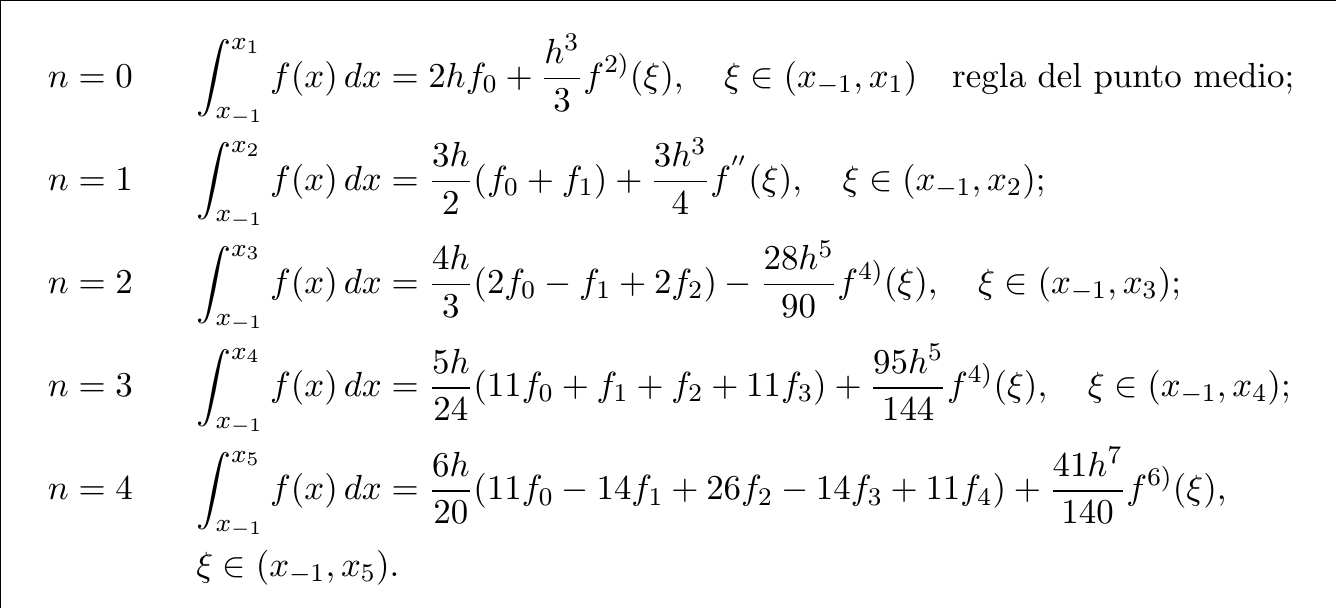
\includegraphics[width=0.95\linewidth]{tema3/formulas-nc-abiertas}
  \end{center}
  Se recomienda, como ejercicio, comprobar estas fórmulas para algunos
  valores de $n$.
\end{example}
\section{Fórmulas de cuadratura compuestas}
\label{sec:fc-compuestas}




%%% Local Variables:
%%% mode: latex
%%% TeX-master: "../apuntes-MNII.tex"
%%% End: 
